%%%%%%%%%%%%%%%%%%%%%%%%%%%%%%%%%%%
%%%  Filename: thesis_template.tex
%%%  ---
%%%  Template for Master Thesis at DTETI UGM   		
%%%  Created using thesisdtetiugm.cls
%%%  --- 
%%%  Written by Canggih Puspo Wibowo
%%%  [canggihpw@gmail.com]
%%%%%%%%%%%%%%%%%%%%%%%%%%%%%%%%%%%

%% Use option "bahasa" or "english" 
%%    to change the basic language used
%% User option "bachelor", "master", or "doctoral"
%% 	  to change the degree
% \documentclass[<bachelor/master/doctoral>,<bahasa/english>]{thesisdtetiugm}
\documentclass[doctoral,bahasa]{thesisdtetiugm}
%======================================
% Information Input
%======================================
% Input author's name and ID number
\author{<<AUTHOR>>}{<<NIM>>}
% Input the thesis' title
\title{<<Thesis title>>}
% Program and the head of the program
\program{<<Program name>>}{<<Program coordinator>>}{<<NIP>>}
% Name of department head and NIP
\departmenthead{<<Head of the department>>}{<<NIP>>}
\major{<<Major>>}
\yearsubmit{<<year submit>>}
\examdate{<<Exam date>>}
% Name of thesis supervisors/promotors
\addsupervisor{<<Supervisor 1>>}{<<NIP>>}
\addsupervisor{<<Supervisor 2>>}{<<NIP>>}
\addsupervisor{<<Supervisor 3>>}{<<NIP>>}
% Name of examiners
\addexaminer{<<Examiner 1>>}{<<NIP 1>>}
\addexaminer{<<Examiner 2>>}{<<NIP 2>>}
\addexaminer{<<Examiner 3>>}{<<NIP 3>>}
\addexaminer{<<Examiner 4>>}{<<NIP 4>>}
\addexaminer{<<Examiner 5>>}{<<NIP 5>>}
\addexaminer{<<Examiner 6>>}{<<NIP 6>>}
\addexaminer{<<Examiner 7>>}{<<NIP 7>>}
\addexaminer{<<Examiner 8>>}{<<NIP 8>>}
\addexaminer{<<Examiner 9>>}{<<NIP 9>>}

%======================================

%% Uncomment block of code below to disable hyphenation
%\tolerance=1
%\emergencystretch=\maxdimen
%\hyphenpenalty=10000
%\hbadness=10000

% Correct bad hyphenation here [example]
\hyphenation{op-tical net-works semi-conduc-tor}

\begin{document}
%======================================
% Create cover etc
%======================================

%---- COVER ----
\printcover{sample/logougm.png}{Pendadaran/Tesis/Ringkasan Tesis*}
% *Choose one

%---- ENDORSEMENT PAGE ----
% Select endorsement page type. If you want to use your own PDF file,  
% 	use \printendorsementpdf, or if you want to use JPG file, use 
% 	\printendorsementjpg. Otherwise, use \printendorsement.
% 	Choose one only. Comment out unused command(s).
%
\printendorsement
%\printendorsementpdf
%\printendorsementjpg{sample/scanned-endorsement.jpg}

%---- DEDICATION PAGE ----
\chapterdedication{contents/dedication/dedication}

%---- STATEMENT PAGE ----
% Select statement page type. If you want to use your own JPG file,  
%	use \chapterstatementjpg{<your *.jpg file path>}. Otherwise, 
%	use \chapterstatement{contents/statement/statement}.
%	Choose one only. Comment out unused command(s).
%
\chapterstatement{contents/statement/statement}
%\chapterstatementjpg{sample/scanned-statement.jpg}

%---- PREFACE PAGE ----
\chapterpreface{contents/preface/preface}

%---- NOMENCLATURE PAGE ----
\chapternomenclature{contents/nomenclature/nomenclature}

%---- ABSTRACT PAGE----
\chapterabstract{contents/abstract/abstract}

%---- INTISARI PAGE----
\chapterintisari{contents/abstract/intisari}
%======================================


%======================================
% Create Table of Contents, List of Figures, List of Tables
% <Do not change this part>
%======================================
\thetoc
\tableofcontents
\thelof
\listoffigures
\thelot
\listoftables
%======================================

%======================================
%  MAIN TEXT
%======================================
\startmain
% You can change 
%    the filename and location of the files inputted
\chapter{Perintah-perintah dasar}


\section{Penggunaan Sitasi}
Contoh penggunaan sitasi \cite{lukito2016,santosa2011user}
\cite{setiawan2014fuzzy} \cite{wibowo2014line} \cite{marenda2016digitory} \cite{wibirama2013dual,wibowo2016clustering}

\section{Penulisan Gambar}

\begin{figure}[h]
	\centering
	\includegraphics[width=10cm]{contents/chapter-1/sample-fig.png}
	\caption{Contoh gambar.}
	\label{Fig: Contoh gambar}
\end{figure}

Contoh gambar terlihat pada Gambar \ref{Fig: Contoh gambar}. Gambar diambil dari \cite{wibowo2016clustering}.

\section{Penulisan Tabel}
\begin{table}[h]
	\caption{tabel ini}
	\vspace{0.5em}
	\centering
	\begin{tabular}{|c|c|c|}
		\hline
		ID & Tinggi Badan (cm) & Berat Badan (kg) \\
		\hline \hline
		A23 & 173 & 62 \\
		A25 & 185 & 78 \\
		A10 & 162 & 70 \\ \hline
	\end{tabular}
	\label{Tab: Tabel Tinggi Berat}
\end{table}
Contoh penulisan tabel bisa dilihat pada Tabel \ref{Tab: Tabel Tinggi Berat}.

\section{Penulisan formula}
Contoh penulisan formula
\begin{equation}
L_{\psi_z} = \{ t_i \mid v_z(t_i) \le \psi_z \}
\end{equation}

Contoh penulisan secara \textit{inline}: $\mathit{PV = nRT}$. Untuk kasus-kasus tertentu, kita membutuhkan perintah "mathit" dalam penulisan formula untuk menghindari adanya jeda saat penulisan formula.

Contoh formula \textbf{tanpa} menggunakan "mathit": $PVA = RTD$

Contoh formula \textbf{dengan} menggunakan "mathit": $\mathit{PVA = RTD}$



\section{Contoh list}
Berikut contoh penggunaan list
\begin{enumerate}
	\item First item
	\item Second item
	\item Third item
\end{enumerate}
\chapter{TINJAUAN PUSTAKA DAN LANDASAN TEORI}


\section{Tinjauan Pustaka}
	Tinjauan pustaka dituliskan berdasar apa yang sudah Anda pelajari dalam rangka penelitian tesis S2. Susunlah tinjauah pustaka dari yang bersifat umum menuju khusus (general to specific). Tinjauan pustaka ini dipelajari dari paper-paper seminar maupun jurnal.
	
\section{Landasan Teori}
	Landasan teori dituliskan berdasar tinjauan pustaka, sebagai bentuk yang lebih spesifik sesuai dengan arah penelitian Anda. Landasan teori ini didapat dari paper maupun buku, yang mendasari metodologi penelitian yang dibahas di Bab III.


\subsection{Penggunaan Sitasi}
Contoh penggunaan sitasi \cite{lukito2016,santosa2011user}
\cite{setiawan2014fuzzy} \cite{wibowo2014line} \cite{marenda2016digitory} \cite{wibirama2013dual,wibowo2016clustering}

\subsection{Penulisan Gambar}

\begin{figure}[h]
	\centering
	\includegraphics[width=10cm]{contents/chapter-2/sample-fig.png}
	\caption{Contoh gambar.}
	\label{Fig: Contoh gambar}
\end{figure}

Contoh gambar terlihat pada Gambar \ref{Fig: Contoh gambar}. Gambar diambil dari \cite{wibowo2016clustering}.

\subsection{Penulisan Tabel}
\begin{table}[h]
	\caption{tabel ini}
	\vspace{0.5em}
	\centering
	\begin{tabular}{|c|c|c|}
		\hline
		ID & Tinggi Badan (cm) & Berat Badan (kg) \\
		\hline \hline
		A23 & 173 & 62 \\
		A25 & 185 & 78 \\
		A10 & 162 & 70 \\ \hline
	\end{tabular}
	\label{Tab: Tabel Tinggi Berat}
\end{table}
Contoh penulisan tabel bisa dilihat pada Tabel \ref{Tab: Tabel Tinggi Berat}.

\subsection{Penulisan formula}
Contoh penulisan formula
\begin{equation}
L_{\psi_z} = \{ t_i \mid v_z(t_i) \le \psi_z \}
\end{equation}

Contoh penulisan secara \textit{inline}: $L_{\psi_z} = \{ t_i \mid v_z(t_i) \le \psi_z \}$.
\chapter{METODOLOGI}

\section{Satu}


\section{Dua}

\chapter{<<Chapter name>>}
\chapter{KESIMPULAN DAN SARAN}

\section{Kesimpulan}

\section{Saran}
%======================================

%======================================
%  References
%======================================
\thereferences
% You can change 
%    the filename and location of the files inputted
\bibliography{references}
%======================================

%======================================
%  Appendix
%======================================
% You can change 
%    the filename and location of the files inputted
\chapterappendix{contents/appendix/appendix}
%======================================

\end{document}